\documentclass[tikz,border=5pt]{standalone}
\usepackage{tikz}
\usetikzlibrary{arrows.meta, calc}
\usetikzlibrary{decorations.markings, arrows}
\usetikzlibrary{decorations.shapes}
\usetikzlibrary{decorations.pathreplacing}

% --- Define Colors ---
\definecolor{myblue}{RGB}{175, 204, 233}
\definecolor{mygreen}{RGB}{125,208,163}

\tikzstyle{blue} = [draw=black,outer sep=0, inner sep=5,
    minimum width=1cm, minimum height=1cm, line width=1,
    top color=myblue, bottom color=myblue, font=\Large, align=center]
\tikzstyle{green} = [draw=black,outer sep=0,inner sep=5,
    minimum width=1cm, minimum height=1cm, line width=1,
    top color=mygreen, bottom color=mygreen, font=\Large, align=center]


\tikzstyle{square} = [draw,outer sep=5,inner sep=3,minimum size=10,
    line width=0, very thick, draw=black!100,
    top color=white,bottom color=white, font=\Huge]
    
\tikzstyle{square2} = [draw,outer sep=5,inner sep=3,minimum size=10,
    line width=0, very thick, draw=black!100,
    top color=white,bottom color=white, font=\Large]
    
\tikzstyle{square3} = [draw=none,outer sep=0,inner sep=0,
    line width=0, color=red!80!black,
    fill=none, font=\Large]


\begin{document}

% ==================================================================
% FIGURE : example 2
% ==================================================================
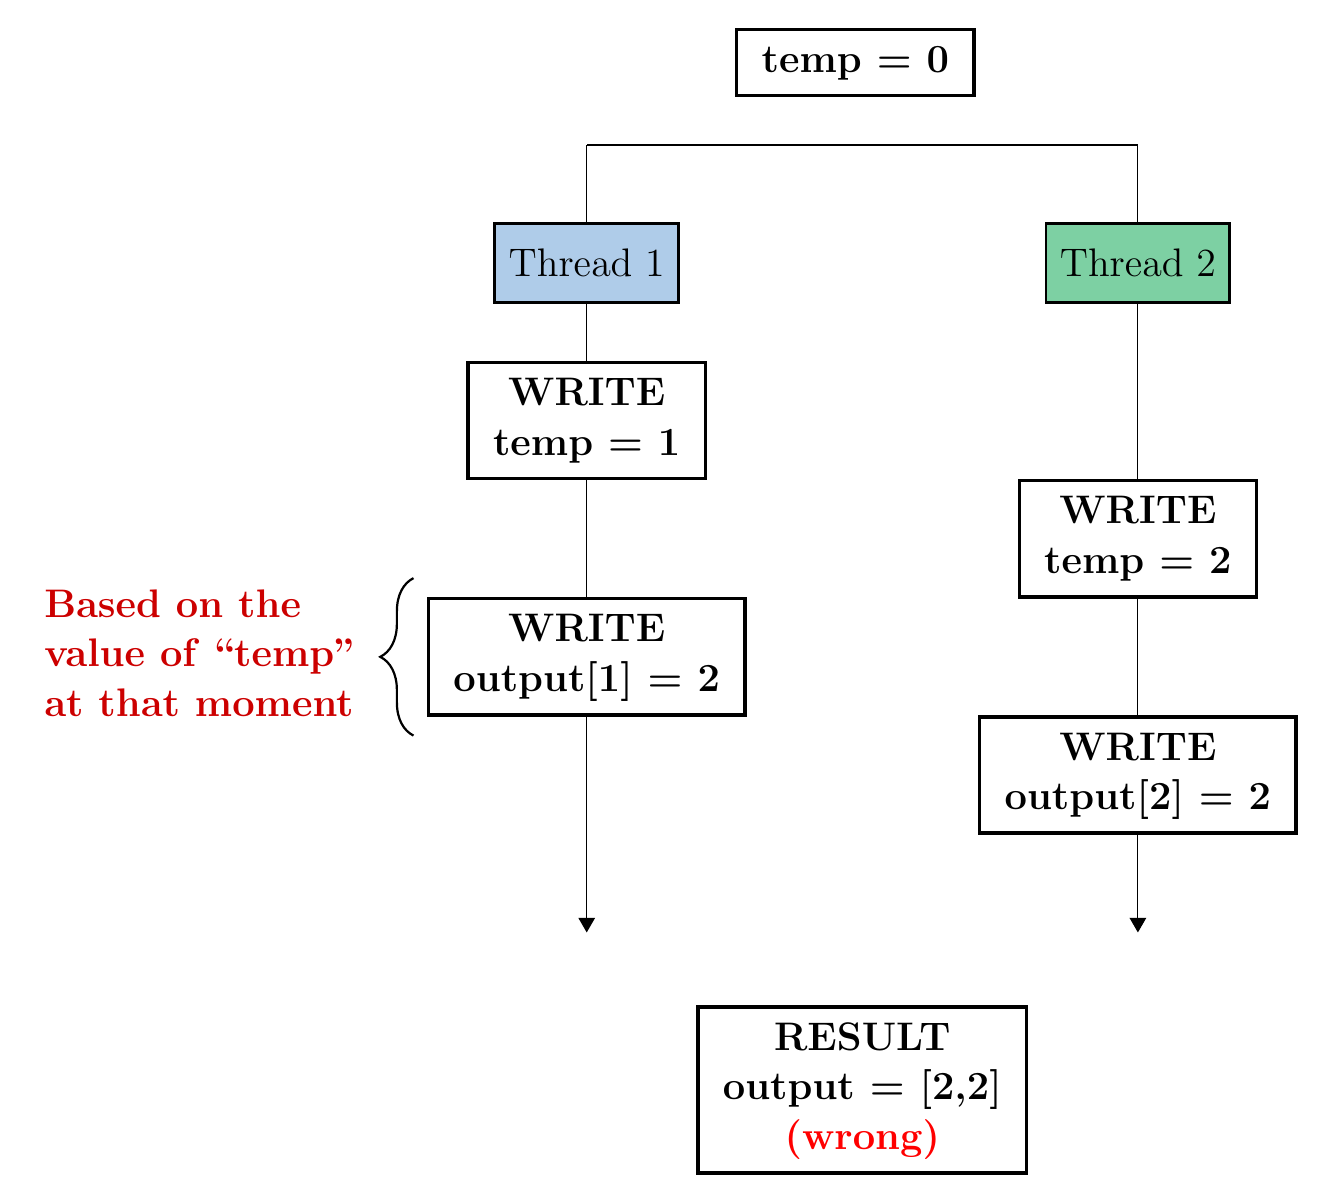
\begin{tikzpicture}


\node[square2] at (-3.0877,7.5478) {\textbf{\begin{tabular}{c} temp = 0 \end{tabular}}};;


\draw[-triangle 60]  (0.5,6.5) -- node[pos=1, anchor=west] {\textbf{\begin{tabular}{c} \end{tabular}}}(0.5,-3.5);
\draw[-triangle 60]  (-6.5,6.5) -- node[pos=1, anchor=west] {\textbf{\begin{tabular}{c} \end{tabular}}}(-6.5,-3.5);
\draw (0.5,6.5) -- (-6.5,6.5);

%%% threads
\node[blue] (t2) at (-6.5,5) {Thread 1};
\node[green] (s2) at (0.5,5) {Thread 2};

\node[square2] at (-6.5,3) {\textbf{\begin{tabular}{c} WRITE \\ temp = 1 \end{tabular}}};
\node[square2] at (-6.5,0) {\textbf{\begin{tabular}{c} WRITE \\ output[1] = 2 \end{tabular}}};


\node[square2] at (0.5,1.5) {\textbf{\begin{tabular}{c} WRITE \\ temp = 2 \end{tabular}}};
\node[square2] at (0.5,-1.5) {\textbf{\begin{tabular}{c} WRITE \\ output[2] = 2 \end{tabular}}};

\node[square2] at (-3,-5.5) {\textbf{\begin{tabular}{c} RESULT \\ output = [2,2] \\ \color{red}{(wrong)} \end{tabular}}};

\draw[decorate,thick, decoration={brace, amplitude=12pt}] (-8.7,-1)--(-8.7,1);
\node[square3,anchor=east] at (-9.2,0) {\textbf{\begin{tabular}{l} Based on the \\ value of  ``temp'' \\ at that moment\end{tabular}}};


\end{tikzpicture}

\end{document}
